\section{Introduction}
Species classification, or taxonomy, is a foundational process in biology that organizes living organisms into a hierarchical structure based on shared traits as shown in Figure~\ref{fig:IVT}. This system provides a universal framework for naming and categorizing species, starting from broad categories and narrowing down to specific groups. Traditionally, taxonomy has relied on observable physical characteristics—such as shape, size, and structural features—for classification. However, with advances in molecular biology and DNA sequencing, genetic information has become a central factor in determining the relationships between organisms. DNA classification offers a precise, data-driven method to analyze genetic similarities and differences, allowing scientists to construct evolutionary lineages and assess genetic relationships more objectively than morphological methods alone. Despite its strengths, DNA-based classification benefits from incorporating morphological and ecological factors, as emphasized by Sosa et al. (2020), to ensure a comprehensive approach to species identification.

\begin{figure*}[t]
\begin{centering}
		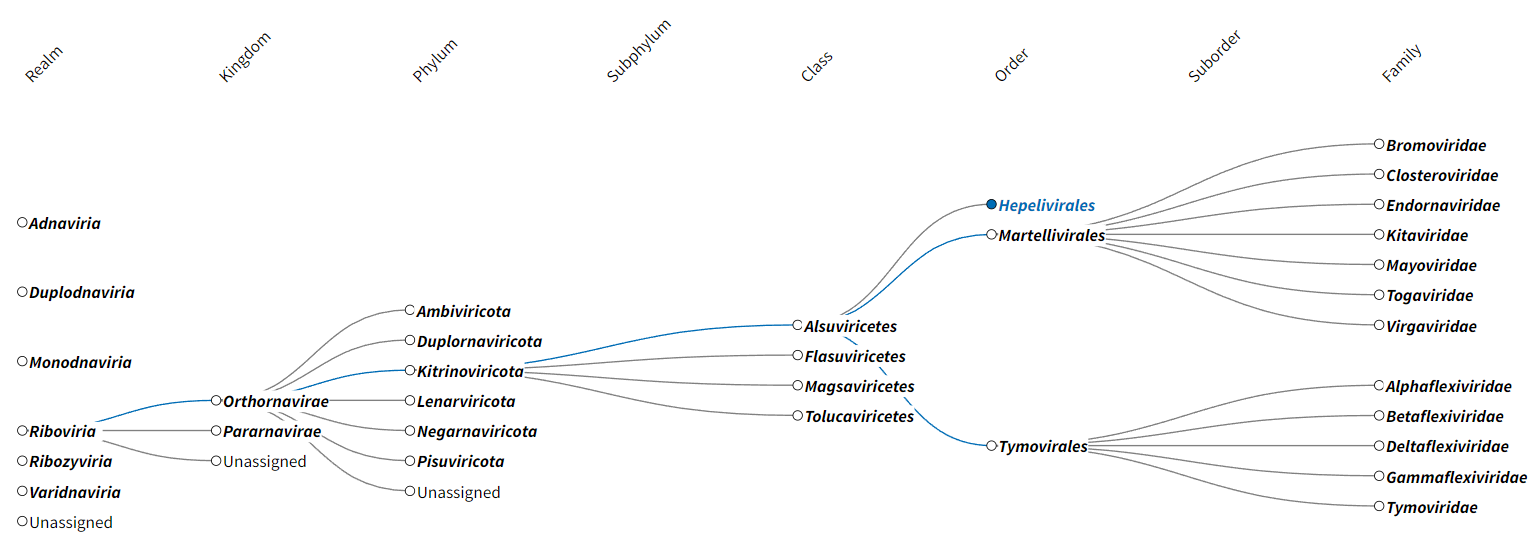
\includegraphics[width=\textwidth]{Figures/heirarchy_IVT.png}
	\caption{distribution  }
\label{fig:IVT}
\end{centering}
\end{figure*}


With the rise of large-scale genetic data, machine learning (ML) has emerged as an invaluable tool for handling complex datasets in taxonomy and genetic research. ML algorithms are capable of learning from data, identifying patterns, and making informed predictions with minimal human oversight. In DNA classification, ML methods enable automation in processes such as DNA sequence segmentation, improving both the speed and accuracy of analysis over traditional manual methods. Algorithms like Support Vector Machines (SVMs) and Artificial Neural Networks (ANNs) are particularly effective for classifying genetic data. ML has applications in identifying genetic variations, discovering evolutionary relationships, and predicting the functional roles of specific genes or genetic elements. It can even identify regions of DNA conserved across multiple species, aiding in evolutionary and biomedical research.

ML-based DNA analysis also has practical applications beyond classification. For instance, by examining genetic variations, researchers can identify specific changes in DNA associated with medical conditions, contributing to diagnostic and therapeutic advancements. ML approaches are also instrumental in examining whole-genome relationships, allowing scientists to uncover evolutionary connections between species. This capability, combined with the ability to quickly adapt to new data, makes ML an essential component of modern genetic research and clinical applications.

In this paper, we present an ML-driven approach for virus classification using DNA sequences, applying a hierarchical classification structure known as Local Classifiers per Node (LCN). Our method classifies viral DNA sequences by leveraging hierarchical relationships to improve classification accuracy. The process begins with data preprocessing, where ambiguous nucleotides—such as M and N—are replaced with the most frequent nucleotide in the sequence. This step ensures consistency across sequences by reducing variability introduced by unidentified bases. After preprocessing, we apply one-hot encoding to represent each nucleotide as a binary vector, preparing the data for input into the ML model.

Due to the limited number of available DNA sequences per virus species, we implement two data augmentation techniques to expand the training dataset. The first method involves adding each sequence's reverse complement to the dataset, effectively doubling the sample size while preserving sequence information. The second method divides each DNA sequence into fixed-length subsequences, further increasing the training data and allowing the model to learn from diverse sequence fragments.

Each encoded subsequence is fed into a one-dimensional convolutional neural network (1D CNN) to extract relevant features. This CNN layer identifies sequence patterns that may be important for classification, capturing relationships within each fragment of the DNA sequence. The CNN output is then passed through a Long Short-Term Memory (LSTM) layer, which captures sequential dependencies within the data, allowing the model to recognize patterns across longer segments of DNA. During prediction, we use soft voting to aggregate the predictions from each subsequence, thereby producing a single classification result for the entire sequence. This voting method enhances accuracy by consolidating information across subsequences.

Our approach achieved an accuracy of 95\%, highlighting the effectiveness of combining hierarchical classification with ML-based feature extraction and sequence analysis. The use of one-hot encoding, data augmentation, and deep learning architectures like CNN and LSTM contributes to the robustness of our classification framework. Our complete methodology, including code and datasets, is accessible on GitHub[2] for reproducibility and further exploration by the research community.

In summary, integrating machine learning into DNA classification opens up new possibilities for taxonomic research, providing tools to analyze and classify genetic sequences with unprecedented speed and precision. This approach not only advances taxonomy but also has broad applications in understanding the roles of genes and proteins in health, disease, and development, bridging the gap between molecular biology and computational science